\clearpage
\thispagestyle{empty}
\section{Контрольная работа 2}



\subsection[2017-2018]{\hyperref[sec:sol_kr_02_2017_2018]{2017-2018}}
\label{sec:kr_02_2017_2018}

\subsubsection*{Минимум}
% 2 + 4 + 14 + 16

\begin{enumerate}
\item Приведите определение условной вероятности случайного события, формулу Байеса.
\item Сформулируйте определение и свойства функции плотности случайной величины.
\item Сформулируйте определение  условного математического ожидания $\E(Y|X=x)$ для совместного дискретного и совместного абсолютно непрерывного распределений.
\item Сформулируйте неравенство Чебышёва и неравенство Маркова.

\item Задана таблица совместного распределения случайных величин $X$ и $Y$.
\begin{center}
\begin{tabular}{lccc}
\toprule
                       & $Y=-1$  & $Y=0$   & $Y=1$   \\
 \midrule
$X=0$                 & $0.2$ & $0.1$ & $0.3$ \\
 $X=1$                 & $0.2$ & $0.1$ & $0.1$ \\
 \bottomrule
\end{tabular}
\end{center}


\begin{enumerate}
    \item Найдите $F_{X,Y}(0, 0)$;
    \item Найдите $\E(X)$, $\E(X^2)$, $\E(Y)$, $\E(Y^2)$;
    \item Найдите $\Var(X)$, $\Var(Y)$;
    \item Найдите $\Cov(X, Y)$, $\Corr(X, Y)$
\end{enumerate}
\item Плотность распределения случайного вектора $(X,Y)$ имеет вид
\[
f_{X,Y}(x,y) =
\begin{cases}
\frac{4x+10y}{7}, & \text{при } (x,y) \in [0;1] \times [0;1] \\
0 , & \text{при } (x,y) \not\in [0;1] \times [0;1] \\
\end{cases}
\]

\begin{enumerate}
\item Найдите $\P(X \leq Y)$;
\item Найдите функцию плотности $f_X(x)$;
\item Найдите $\E(X)$, $\E(Y)$ и $\Cov(X, Y)$;
\item Являются ли случайные величины $X$ и $Y$ независимыми?
\end{enumerate}


\end{enumerate}

\subsubsection*{Задачи}

\begin{enumerate}[resume]

\item Статистика авиакомпании «А» за много лет свидетельствует о том, что 10\% людей, купивших билет на самолет, не являются на рейс. Авиакомпания продала 330 билетов на 300 мест.
\begin{enumerate}
\item Какова вероятность, что всем явившимся на рейс пассажирам хватит места?
\item Укажите наибольшее число билетов, которое можно продавать на 300 мест, чтобы случаи переполнения случались не чаще, чем на одном из десяти рейсов.
\end{enumerate}

\item Сегодня акция компании «Ух» стоит 1 рубль. Каждый день акция может с вероятностью 0.7 вырасти на 1\%, с вероятностью 0.2999 упасть на 1\% и с вероятностью 0.0001 обесцениться (упасть на 100\%).
\begin{enumerate}
\item Считая изменение цены акции независимыми, найдите математическое ожидание её стоимости через 20 торговых дней.
\item Найдите предел по вероятности среднего изменения цены акции в процентах на бесконечном промежутке времени (Ответ обоснуйте).
\item Найдите математическое ожидание цены акции на бесконечном промежутке времени.
\item Инвестор вложил все свои средства в акции компании «Ух». Найдите вероятность его разорения на бесконечном промежутке времени.
\end{enumerate}
\end{enumerate}


\newpage
\subsection[2016-2017]{\hyperref[sec:sol_kr_02_2016_2017]{2016-2017}}
\label{sec:kr_02_2016_2017}


\textbf{Неравенства Берри–Эссеена:} Для любых $n \in \mathbb{N}$ и всех $x \in \mathbb{R}$ имеет место оценка:
\[
    \bigl|F_{S_n^{*}}(x) - \Phi(x)\bigr| \leq 0.48 \cdot \frac{\E(|\xi_i - \E\xi_i|^3)}{\Var^{3/2}(\xi_i)\cdot\sqrt{n}} \text{,}
\]
где $\Phi(x) = \int_{-\infty}^{x}\frac{1}{\sqrt{2\pi}}e^{-\frac{t^2}{2}}\,dt$, \; $S_n^* = \frac{S_n - \E(S_n)}{\sqrt{\Var(S_n)}}$, \; $S_n = \xi_1 + \ldots + \xi_n$

\textbf{Распределение Пуассона:} Случайная величина $\xi$ имеет распределение Пуассона с параметром $\lambda > 0$,  если она принимает целые неотрицательные значения с вероятностями $\P(\{\xi = k\}) = \frac{\lambda^k}{k!}e^{-\lambda}$. Приличным студентам должно быть известно, что в этом случае $\E(\xi) = \Var(\xi) = \lambda$.

\begin{enumerate}
\item Пусть $\E(\xi) = 1$, $\E(\eta) = -2$, $\Var(\xi) = 1$, $\E(\eta^2) = 8$, $\E(\xi \eta) = -1$. Найдите
\begin{enumerate}
\item $\E(2\xi-\eta+1)$, $\Cov(\xi, \,\eta)$, $\Corr(\xi, \,\eta)$,  $\Var(2\xi-\eta+1)$;
\item $\Cov(\xi+\eta, \,\xi+1)$, $\Corr(\xi+\eta, \,\xi+1)$, $\Corr(\xi+\eta-24, \,365 - \xi - \eta)$, $\Cov(2016\cdot\xi, \, 2017)$.
\end{enumerate}

\item
Совместное распределение доходностей акций двух компаний задано с помощью таблицы:

\begin{center}
\begin{tabular}{ccc}
\toprule
         & $\eta=-1$ & $\eta=1$ \\
\midrule
$\xi=-1$  & $0.1$       & $0.2$   \\
$\xi=0$   & $0.2$       & $0.2$   \\
$\xi=2$   & $0.2$       & $0.1$   \\
\bottomrule
\end{tabular}
\end{center}

\begin{enumerate}
  \item Найдите частные распределения случайных величин $\xi$ и $\eta$.
  \item Найдите $\Cov(\xi,\,\eta)$.
  \item Сформулируйте определение независимости дискретных случайных величин.
  \item Являются ли случайные величины $\xi$ и $\eta$ независимыми?
  \item Найдите условное распределение случайной величины $\xi$, если $\eta = 1$.
  \item Найдите условное математическое ожидание случайной величины $\xi$, если $\eta = 1$.
  \item Найдите математическое ожидание и дисперсию величины $\pi = 0.5\, \xi + 0.5\, \eta$.
  \item Рассмотрим портфель, в котором $\alpha$ — доля акций с доходностью $\xi$ и $(1 - \alpha)$ — доля акций с доходностью $\eta$. Доходность этого портфеля есть случайная величина
  \[\pi(\alpha) = \alpha \xi + (1-\alpha)\eta.\]
  Найдите такую долю $\alpha \in [0;\,1]$, при которой доходность портфеля $\pi(\alpha)$ имеет наименьшую дисперсию.
\end{enumerate}

\item Число посетителей сайта \url{pokrovka11.wordpress.com} за один день имеет распределение Пуассона с математическим ожиданием 250.
\begin{enumerate}
  \item Сформулируйте неравенство Маркова. При помощи данного неравенства оцените вероятность того, что за один день сайт посетят более 500 человек.
  \item Сформулируйте неравенство Чебышева. Используя данное неравенство, определите наименьшее число дней, при котором с вероятностью не менее 99\% среднее за день число посетителей будет отличаться от 250 не~более чем на 10.
  \item Решите предыдущий пункт с помощью центральной предельной теоремы.
  \item Сформулируйте закон больших чисел. Обозначим через $\xi_i$ число посетителей сайта за $i$-ый день. Найдите предел по вероятности последовательности $\frac{\xi_1^2 + \ldots + \xi_n^2}{n}$ при $n \rightarrow \infty$.
\end{enumerate}

\item Отведав медовухи, Винни–Пух совершает случайное блуждание на прямой. Он стартует из начала координат и в каждую следующую минуту равновероятно совершает шаг единичной длины налево или направо. Передвижения Винни-Пуха схематично изображены на следующем рисунке.
\begin{figure}[h]
    \noindent\centering{
    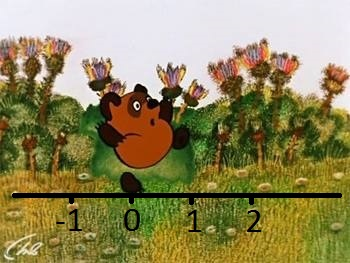
\includegraphics[width=80mm]{images/Winnie_the_Pooh_and_Medovuh.jpg}
    }
    \caption{Случайные бродилки.}
    \label{wun762hkej}
\end{figure}
\begin{enumerate}
  \item Сформулируйте центральную предельную теорему.
  \item При помощи центральной предельной теоремы оцените вероятность того, что ровно через час блужданий Винни-Пух окажется в области $(-\infty; \, -5]$.
  \item Используя неравенство Берри–Эссеена оцените погрешность вычислений предыдущего пункта.
\end{enumerate}


\item
Cлучайные величины $\xi$ и $\eta$ означают время безотказной работы рулевого управления и двигателя автомобиля соответственно. Время измеряется в годах. Совместная плотность имеет вид:
\[
f_{\xi, \,\eta}(x,\,y) =
\begin{cases}
0.005\,e^{-0.05\,x-0.1\,y} & \text{ при } x > 0, y > 0, \\
0                    & \text{ иначе.}
\end{cases}
\]

\begin{enumerate}
  \item Найдите частные плотности распределения случайных величин $\xi$ и $\eta$.
  \item Являются ли случайные величины $\xi$ и $\eta$ независимыми?
  \item Найдите вероятность того, что двигатель прослужит без сбоев более пяти лет.
  \item Найдите вероятность того, что двигатель прослужит без сбоев более восьми лет, если он уже проработал без сбоев три года.
  \item Найдите условное математическое ожидание безотказной работы рулевого управления, если двигатель проработал без сбоев пять лет,  $\E(\xi | \eta = 5)$.
  \item Найдите вероятность того, что рулевое управление проработает без сбоев на два года больше двигателя,  $\P(\{\xi - \eta > 2\})$.
\end{enumerate}

\item Бонусная задача

Случайная величина $\xi$ имеет плотность распределения
\[
    f_{\xi}(x) = \frac{1}{2} \cdot \frac{1}{\sqrt{2\pi}}e^{-\frac{(x-1)^2}{2}} + \frac{1}{2} \cdot \frac{1}{\sqrt{2\pi}}e^{-\frac{(x+1)^2}{2}} \text{.}
\]

\begin{enumerate}
\item Найдите $\E(\xi)$, $\E\left(\xi^2\right)$, $\Var(\xi)$.
\item Покажите, что функция $f_{\xi}(x)$, действительно, является плотностью распределения.
\end{enumerate}
\end{enumerate}



\subsection[2015-2016]{\hyperref[sec:sol_kr_02_2015_2016]{2015-2016}}
\label{sec:kr_02_2015_2016}




Продолжительность: 1 час 20 минут

\begin{enumerate}
\item Функция плотности случайного вектора $\xi=(\xi_1, \xi_2)^T$ имеет вид
\[
f(x,y)=\begin{cases}
0.5x + 1.5y, \text{ если } 0<x<1, \; 0<y<1 \\
0, \text{ иначе }
\end{cases}
\]
Найдите:
\begin{enumerate}
\item Математическое ожидание $\E(\xi_1 \cdot \xi_2)$
\item Условную плотность распределения $f_{\xi_1|\xi_2} (x|y)$
\item Условное математическое ожидание $\E(\xi_1| \xi_2=y)$
\item Константу $k$, такую, что функция $h(x,y)=kx\cdot f(x,y)$ будет являться совместной функцией плотности некоторой пары случайных величин
\end{enumerate}

\item На курсе учится очень много студентов. Вероятность того, что случайно выбранный студент по результатам рубежного контроля имеет хотя бы один незачет равна $0.2$. Пусть $\xi$ и $\eta$ — число студентов с незачетами и без незачетов в случайной группе из $10$ студентов. Найдите $\Cov(\xi,\eta)$, $\Corr(\xi,\eta)$, $\Cov(\xi-\eta,\xi)$. Являются ли случайные величины $\xi-\eta$ и $\xi$ независимыми?

\item Доходности акций компаний А и В – случайные величины $\xi$ и $\eta$. Известно, что $\E(\xi)=1$, $E(\eta)=1$, $\Var(\xi)=4$, $\Var(\eta)=9$, $\Corr(\xi,\eta)=-0.5$. Петя принимает решение потратить свой рубль на акции компании А, Вася — 50 копеек на акции компании А и 50 копеек на акции компании В, а Маша  принимает решение вложить свой рубль в портфель $R=\alpha\xi+(1-\alpha)\eta$, $(0 \leq \alpha \leq 1)$, обладающий минимальным риском. Найдите $\alpha$, ожидаемые доходности и риски портфелей Пети, Васи и Маши.

\item Будем считать, что рождение мальчика и девочки равновероятны.
\begin{enumerate}
\item Оцените с помощью неравенства Маркова вероятность того, что среди тысячи новорожденных младенцев, мальчиков будет более 75\%.
\item Оцените с помощью неравенства Чебышёва вероятность того, что доля мальчиков среди тысячи новорожденных младенцев будет отличаться от 0.5 более, чем на 0.25
\item С помощью теоремы Муавра-Лапласа вычислите вероятность из предыдущего пункта.
\end{enumerate}

\item Сейчас валютный курс племени «Мумба» составляет 100 оболов за один рубль. Изменение курса за один день — случайная величина $\delta_i$ с законом распределения:

\begin{center}
\begin{tabular}{lrrr}
\toprule
$x$ & $-1$ & $0$ & $2$ \\ \midrule
$\P(\delta_i = x)$ & $0.25$ & $0.5$ & $0.25$ \\
\bottomrule
\end{tabular}
\end{center}

Найдите вероятность того, что через полгода (171 день) рубль будет стоить более 250 оболов, если ежедневные изменения курса происходят независимо друг от друга.

\item \textbf{Бонусная задача}

Число посетителей, зашедших в магазин в течении дня — пуассоновская случайная величина с параметром $\lambda$. Каждый из посетителей совершает покупку с вероятностью $p$, не зависимо от других посетителей. Найдите математическое ожидание числа человек, совершивших покупку.

\end{enumerate}
